\documentclass{article}
\usepackage{ctex}
\usepackage{verbatim}
\usepackage{listings}
\usepackage[left=1in,right=1in,top=0.7in,bottom=0.7in]{geometry}
\twocolumn

\usepackage{tikz}
\usetikzlibrary{shapes,arrows}
\tikzstyle{r} = [rectangle, minimum width=2cm, minimum height=1cm, text centered, draw=black]

\title{人工智能作业}
\author{骆天奇\\2016254060407}
%\date{19.11.6}
\date{\today}

\begin{document}
	\maketitle
	\section{semantic networks}
	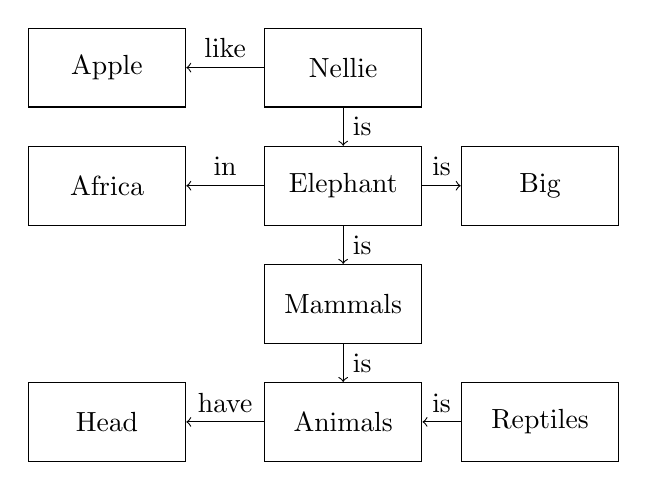
\begin{tikzpicture}[node distance = 1.5cm]
		\node[r](nellie){Nellie};
		\node[r,below of=nellie](ele){Elephant};
		\node[r,left of=nellie, xshift=-1.5cm](apple){Apple};
		\node[r,left of=ele, xshift=-1.5cm](africa){Africa};
		\node[r,right of=ele, xshift=1cm](big){Big};
		\node[r,below of=ele](mammals){Mammals};
		\node[r,below of=mammals](animals){Animals};
		\node[r,left of=animals, xshift=-1.5cm](head){Head};
		\node[r,right of=animals, xshift=1cm](reptiles){Reptiles};
		
		\draw[->](nellie)--node[right]{is}(ele);
		\draw[->](nellie)--node[above]{like}(apple);
		\draw[->](ele)--node[right]{is}(mammals);
		\draw[->](ele)--node[above]{in}(africa);
		\draw[->](ele)--node[above]{is}(big);
		\draw[->](mammals)--node[right]{is}(animals);
		\draw[->](reptiles)--node[above]{is}(animals);
		\draw[->](animals)--node[above]{have}(head);
	\end{tikzpicture}
	\section{汉诺塔结果}
		\verbatiminput{out.txt}
	\section{汉诺塔代码}
		\verbatiminput{hannuota.py}
	
\end{document}
